\chapter{Background}
\label{chapter:background} 

\section{Electricity consumption of ICT equipments}
\label{section:ictequipment} 
ICT equipments consume a significant amount of electricity. A survey conducted by Heddeghem et al. \cite{DBLP:journals/comcom/HeddeghemLLCPD14} shows the electricity consumption and growth trends of three classes of ICT equipments: personal computers, communication networks, and data centers. Personal computers include equipments such as desktop, laptop and external monitors. Communication networks includes residential network access equipments (such as WiFi routers and modems), network equipments used in offices (such as routers and switches) and telecom-operator network equipments (such as base stations, routers and optical amplification systems). Data-centers house storage and computing servers, communication network equipments, and power provisioning and cooling facilities.  In this classification there are overlaps, for instance, telcom operator can have office network equipments and data-centers. After carefully avoiding possible redundant measurements, the researchers estimated absolute electricity consumption and annual consumption growth rate of each category of equipments for the period 2007 and 2012. The results of the study show that the global electricity consumption of ICT equipments in all the three categories combined contributed 3.9\% in 2007 and 4.6\% in 2012. The estimated annual growth rate of the individual category is 5\% for personal computers, 10\% for communication networks, and 4\% for data-centers. These growth rates are higher than that of the total global electricity consumption, which is 3\%.

\section {Data-center electricity consumption}
\label{section:datacenter} 
In Section~\ref{section:ictequipment} we described data-center's global share in electricity consumption. In this section we describe the components involved within the data center itself.

Electricity consumption units with in a typical data-center can be classified into two broad groups \cite{DBLP:journals/comsur/DayarathnaWF16}: The first group is IT equipments (which includes computing servers, storage servers and networking components) and the other group is infrastructure facilities (which includes power provisioning, cooling and lighting components).

Figure~\ref{fig:datacenterenergy} \cite{DBLP:journals/comsur/DayarathnaWF16} shows the electricity consumption proportion of the data-center components. This value differs significantly from one data-center to another \cite{DBLP:series/synthesis/2013Barroso}, for instance, due to architectural difference\cite{DBLP:conf/eenergy/GyarmatiT10} or energy efficiency of the components. The infrastructure facility components take the large proportion (65\%) of the consumption. 

\begin{figure}[ht]
	\begin{center}
		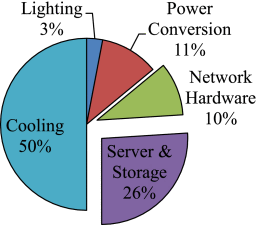
\includegraphics[width=6cm]{images/datacenterenergy.png}
		\caption{Energy consumption percentage of data-center components}
		\label{fig:datacenterenergy}
	\end{center}
\end{figure}
Though the infrastructure facility consumes relatively larger amount of electricity, the focus of this study is on the IT equipment components, particularly on the network equipments. 

If we further zoom in on the IT equipments part, we can find server, storage and network equipments. A data-center servers consist of one or more CPU cores, memory and I/O devices. The energy consumption relationship among these components is shown in Figure~\ref{fig:serverenergy}. Combined, Memory and CPU units consume the larger amount of energy relative to other components. The fact that CPU is the dominant electricity consuming unit is exploited by Fan et al. in \cite{DBLP:conf/isca/FanWB07} to model the dynamic power usage of thousands of servers by using only CPU utilization as a parameter. The result of their study was very accurate, with error as low as 1\%. 
\begin{figure}[ht]
	\begin{center}
		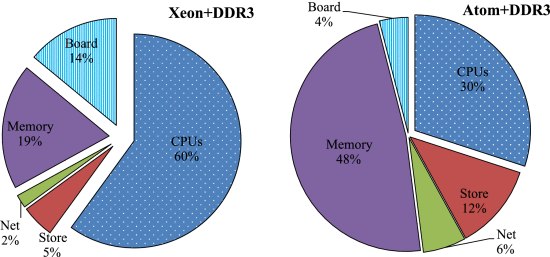
\includegraphics[width=8cm]{images/serverenergy.png}
		\caption{Energy consumption percentage of Xeon based (on the left) and Atom based (on the right) servers}
		\label{fig:serverenergy}
	\end{center}
\end{figure}
\section{Energy proportionality}
\label{section:energyproportionality}
The only reason the study of energy consumption management of network equipment becomes so important is that, in general, ICT equipments do not consume energy proportional to their workload. An ideal ICT equipment is the one which consume zero electricity when it is idle, and it consumes electricity proportional to its workload when it is active. However, the reality is, even power efficient servers consume about 50\% of their peak power \cite{DBLP:journals/computer/BarrosoH07}, even when they are doing nothing. This percentage can even reach 85\% for network switches \cite{DBLP:conf/IEEEcloud/FiandrinoKBZ15}. Figure~\ref{fig:energyproportionality} in \cite{DBLP:conf/networking/MahadevanSBR09} shows the energy proportionality of a typical network equipment. From the graph we can observe that the dynamic power consumption range is narrow.
\begin{figure}[ht]
	\begin{center}
		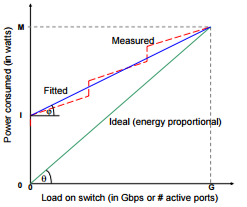
\includegraphics{images/energyproportionality.png}
		\caption{Ideal and measured energy proportionality of a network equipment}
		\label{fig:energyproportionality}
	\end{center}
\end{figure}
Three approaches are in common use to deal with this situation. The first one is re-engineering network devices so as to make them more energy proportional, device vendors are the prime role player in this aspect. The second approach is related to the operating rate of a network equipment port. A typical switch can operate on different transmission rate (100Mbps, 1 Gbps or 10 Gbps). An active port transmitting at 10 Gbps can consume more energy than if it transmit at 100 Mbps. Rate adaptation is the approach devised to take advantage of this situation. Instead of transmitting at the maximum rate all time,  the network port can be made to adapt to the actual traffic load. This energy saving approach is known as Adaptive Link Rate (ALR). The third approach, which is known as Low Power Idle (LPI), allows a network device to send data as fast as possible and then enter low power mode between transfers. The low power mode can further be extended by a technique called packet coalescing, which allows more energy saving \cite{DBLP:journals/comsur/BollaBDC11}. 
\section{Packet-level and flow-level Simulators}
\label{section:packetflow} 
Packet-level simulators strives to model a given network phenomenon at the granularity level of packets, thus in general they are accepted by the research community to be more accurate compared to flow-level simulators \cite{DBLP:journals/jpdc/CasanovaGLQS14}. One of the most popular packet-level simulator is NS-3, which is categorized under discrete-event simulator with events corresponding to sending and receiving packets \cite{ns3}. Though packet-level simulators tend to be more accurate, they fail to scale well in the area of large-scale networks. 

In the area of large-scale networks, flow-level simulators are the preferred alternative. Rather than modeling a given network phenomenon at a packet level, flow-level simulators treat a set of packets as a single unit \cite{DBLP:journals/jpdc/CasanovaGLQS14}. The most commonly used definition for flow in the context of computer networking is coined by Claffy et al. in \cite{claffy1998nature}: 

``\ldots a flow \ldots a unidirectional traffic stream with a unique [source-IP-address, source-port, destination-IP-address, destination-port, IP-protocol] tuple \ldots''

In addition to the five tuple mentioned in the definition, a flow also has a limited time duration. Claffy et al. used a time limit of 64 seconds as a flow duration in their study. Researchers such as Carneiro et al. \cite{DBLP:conf/valuetools/CarneiroFR09}, adopted this same definition to develop flow monitoring module for NS-3, a module that can generate information such as amount of packets or bytes transferred, packets dropped or transmission start and end time for each flow. Barakat et al. in \cite{DBLP:journals/tsp/BarakatTIDO03} also used the same definition to model traffic at the flow-level for the Internet backbone link. By abstracting away fine details, flow-level models provides easy way to instantiate experiments and they also scale very well for conducting large-scale network simulations \cite{DBLP:journals/jpdc/CasanovaGLQS14,DBLP:journals/tsp/BarakatTIDO03}.
\section{Simulating and modeling energy consumption of large-scale networks}
One way of conducting energy consumption or any other experiment is to use real production environment or test-bed environment, both are referred to as \emph{in vivo} in  \cite{DBLP:journals/jpdc/CasanovaGLQS14}. In the former case, handling transient and varying conditions would make the data collection and prediction very difficult and often times, a production environment is not available for experimentation. In the later case, it requires setting-up a separate testing environment designed solely for the purpose of conducting the desired experiment. This approach apart from being expensive, it requires significant amount of time for experiment setup and, it is also non-repeatable as experimenting with different scenario demands a modified or new configuration.

The other alternative for experimenting is simulation, also referred to as \emph{in silico} in \cite{DBLP:journals/jpdc/CasanovaGLQS14}. Simulation, unlike real environment, allows great flexibility in terms of experiment configuration, control and repetition. In addition it can also be less time consuming and less expensive.That is why virtually in all computer network related researches simulations are widely used. 

In this study we simulate energy-aware large scale distributed networks using SimGrid (Detail description about SimGrid follows in the next section). When we say large-scale distributed network, we are referring to a set of networks residing inside in the distributed data centers and also the networks that are used to connect them. 

The energy consumption E of an equipment depends on the operating power P at time t. The total energy consumption for a time period T is given by equation (2.1) \cite{DBLP:conf/wowmom/OrgerieLLL11}. 
\begin{equation}
  E(T) = \int_{0}^{T} P(t) dt
\end{equation} 
Due to the energy proportionality characteristic described in Section~\ref{section:energyproportionality}, the common approach used to compute the energy consumption is to divide the power component into two parts: static/idle power (\($$P_{static}$$\)) and dynamic power (\($$P_{dynamic}$$\)) as shown in equation (2.2). Then the total energy is obtained by multiplying the total power, \($$P_{total}$$\) by the time duration \cite{DBLP:conf/wowmom/OrgerieLLL11,DBLP:journals/tjs/KliazovichBK12,DBLP:conf/networking/MahadevanSBR09,DBLP:journals/comsur/DayarathnaWF16}. 
\begin{equation}
 P_{total} = P_{static} + P_{dynamic}
\end{equation} 
For a typical network equipment such as a switch, the static part constitutes the power consumption of the chassis and the line-cards (when all the ports on the line-cards are switched off). The dynamic part, on the other hand, constitutes the power consumption of the switch ports running at a given rate multiplied by the utilization factor \cite{DBLP:conf/networking/MahadevanSBR09}. Equation (2.3) shows how to compute the total power for a switch, where \($$P_{switch}$$\), is the total power consumption of a switch, \($$P_{chassis}$$\) and \($$P_{linecard}$$\) is the power consumption of the chassis and the line card, respectively. \($$P_{rate}$$\), is the power consumption of a given port at a given rate and \($$numports_{rate}$$\) is the number of ports running at a given rate. The rate can take any value such as 10 Mbps, 100 Mbps, 1 Gbps or 10 Gbps.
\begin{equation}
\begin{split}
P_{switch} &= P_{chassis} + (numlinecards \times P_{linecard})  + \\
&\sum_{rate=min}^{max} (numports_{rate} \times P_{rate} \times utilizationFactor)
\end{split}
\end{equation}
\section{SimGrid}
Figure~\ref{fig:SimGrid} shows the structure of SimGrid and how its core works. The top three components are the APIs that users can use to develop their simulation. Both MSG and SMPI are used to specify simulated applications as concurrent processes. The difference is that using MSG, users can simulate any arbitrary application, whereas, using SMPI users can simulating existing MPI applications, the MPI processes are created automatically from C or Fortran MPI programs. SIMDAG, on the other hand, does not use concurrent processes. It allows users to describe their application as communicating task graph. The next layer, SIMIX, implements the mechanisms that are required to simulate the concurrent process of MSG and SMPI applications. It also provides process control and synchronization functionalities. The bottom layer, SURF, is the simulation core, it simulates the execution of activities on computing or communication resources \cite{DBLP:journals/jpdc/CasanovaGLQS14}.

\begin{figure}[ht]
	\begin{center}
		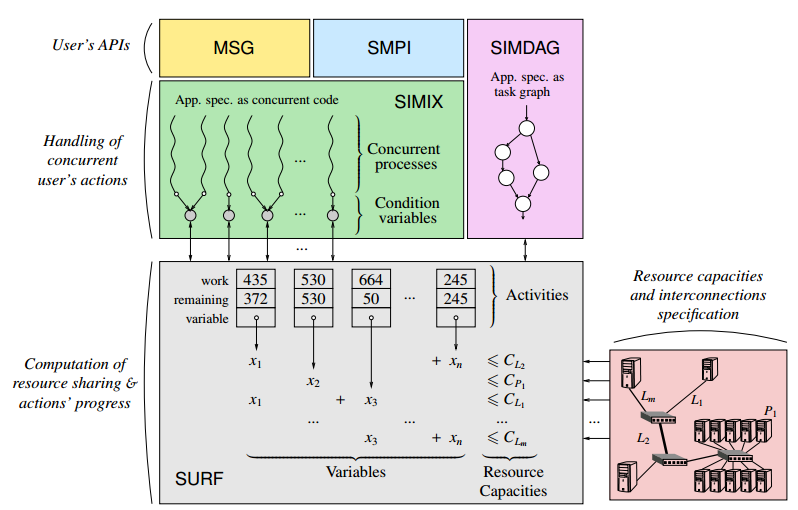
\includegraphics[width=14cm]{images/SimGrid.png}
		\caption{Architecture of SimGrid}
		\label{fig:SimGrid}
	\end{center}
\end{figure}
In SimGrid for each simulated activity, such as computation or data transfer, there is a corresponding condition variable, in Figure~\ref{fig:SimGrid} it is shown in SIMIX box. This condition variable synchronizes the concurrent processes of the simulated applications. The computing (\($$P_{x}$$\)) and the communication (\($$L_{x}$$\)) resources are shown on the bottom-right side of the figure. Computing resources are defined in terms of computing power, whereas, communication resources are defined in terms of bandwidth and latency. As shown in the SURF box, multiple activities can share the same resource (e.g. (\($$x_{1}$$\), \($$x_{n}$$\)), (\($$x_{1}$$\), \($$x_{3}$$\)) or (\($$x_{3}$$\), \($$x_{n}$$\))) or one activity can use multiple resources (e.g. \($$x_{1}$$\) or \($$x_{3}$$\) or  \($$x_{n}$$\)). Activities that share the same resource are limited by the capacity of that resource. Each activity is defined by the total and remaining work to be executed. When the work associated with the activity completes, the corresponding upper layer components receive a notification signal \cite{DBLP:journals/jpdc/CasanovaGLQS14}.

As we have already discussed in Section~\ref{section:packetflow}, the advantages of flow-level simulation is scalability in terms of speed and memory usage. This is a good opportunity .

\section{Related Simulators}